\chapter{Pattern GoF}
\label{GoF}

\section{Design Pattern GoF}

\dfn{Pattern GoF}{
    I \newfancyglitter{pattern GoF} (Gang of Four) sono un insieme di 23 pattern 
    di progettazione software, descritti nel libro \textit{Design Patterns: Elements of Reusable Object-Oriented Software}
    di Erich Gamma, Richard Helm, Ralph Johnson e John Vlissides (vengono mostrati in C++, analizzando
    dei progetti di successo e delle soluzioni a problemi ricorrenti).
    Si dividono in tre categorie: creazionali, strutturali e comportamentali.
}

\cor{GRASP e GoF}{
    I \fancyglitter{pattern GoF} sono degli "schemi di progettazione avanzata",
    mentre i \fancyglitter{pattern GRASP} sono dei principi di progettazione.
}

\clm{}{}{
    I pattern GoF preferiscono la composizione all'ereditarietà. Il meccanismo
    di delega rende la composizione potente quanto l'ereditarietà.
    \paragraph{Ereditarietà tra classi:}
    \begin{itemize}
        \item [$\Rightarrow$] Si definisce un oggetto in termini di un altro;
        \item [$\Rightarrow$] Riuso \fancyglitter{White-box}, ossia la visibilità
        della superclasse è la visibilità della sottoclasse;
        \item [$\Rightarrow$] Definità \fancyglitter{staticamente}, non è possibile 
        cambiarla a tempo di esecuzione;
        \item [$\Rightarrow$] Una modifica alla sopraclasse può avere effetti
        collaterali sulle sottoclassi (non viene rispettato l'incapsulamento).
    \end{itemize}

    \paragraph{Composizione tra oggetti:}
    \begin{itemize}
        \item [$\Rightarrow$] Le funzionalità sono ottenute assemblando e componendo
        gli oggetti per avere funzionalità più complesse;
        \item [$\Rightarrow$] Riuso \fancyglitter{Black-box}, ossia i dettagli
        interni non sono conosciuti;
        \item [$\Rightarrow$] Se una classe ne usa un'altra questa può essere referenziata
        come un'interfaccia, quindi è possibile cambiare l'implementazione a tempo di esecuzione;
        \item [$\Rightarrow$] Utilizzando un'interfaccia si rispetta l'incapsulamento per cui solo
        una modifica all'interfaccia può avere effetti collaterali.
    \end{itemize}
}

\nt{In questo corso se ne esamineranno solo 9.}

\dfn{Polimorfismo}{
    Le sottoclassi possono essere castate in base al tipo, 
    nascondendo alcuni dettagli al cliente.
}

\dfn{Specializzazione}{Le sottoclassi
    guadagnano funzionalità aggiuntive rispetto alla superclasse.}

\nt{La dicitura $<<$stereotipe$>>$ (o $<<$stereotype$>>$) indica che non si fa riferimento a nomi di classi.
    Si tratta di metaclassi.}

\section{Pattern Creazionali}

\dfn{Pattern Creazionali}{
    I \newfancyglitter{pattern creazionali} risolvono problematiche inerenti
    l'istanziamento degli oggetti.
}

\subsection{Abstract Factory}

\mypattern{Abstract Factory}{

    \paragraph{Problema:} Come creare famiglie di classi correlate che implementano
    un'interfaccia comune?

    \paragraph{Soluzione:} Definire un'interfaccia \textbf{Factory} (astratta).
    Definire una classe \textbf{Factory} concreta per ogni famiglia di elementi da creare.
    Opzionalmente si può definire una classe astratta che implementi l'interfaccia
    factory e fornisce servizi comuni alle factory che la estendono.

}

\clm{}{}{
    \begin{itemize}
        \item [$\Rightarrow$] Presenta un'interfaccia per la creazione di famiglie
        di prodotti;
        \item [$\Rightarrow$] Il cliente può creare prodotti vincolati tra loro;
        \item [$\Rightarrow$] È possibile cambiare la famiglia di prodotti senza
        modificare il codice del cliente;
        \item [$\Rightarrow$] È possibile creare una classe AbstractFactory a cui
        si accede tramite un Singleton;
        \item [$\Rightarrow$] È usato nelle librerie Java per la creazione di famiglie GUI
        per diversi SO o sottosistemi GUI.
    \end{itemize}
}

\cd{
    \begin{center}
        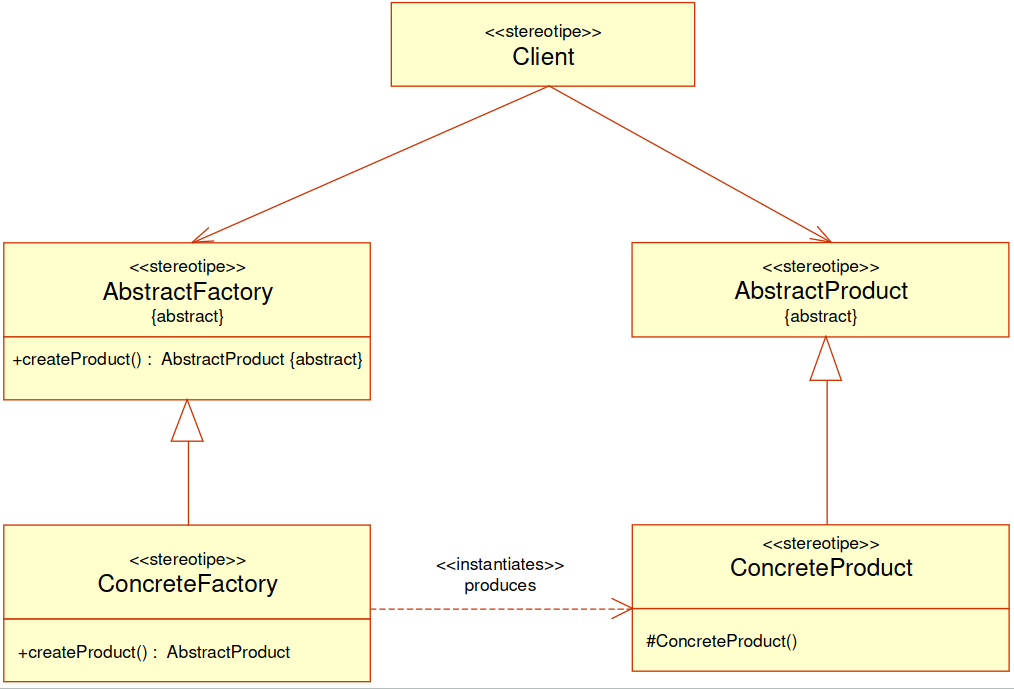
\includegraphics[scale=0.43]{images/AbstractFactory.png}
    \end{center}
    
}

\ex{Applicazione di Abstract Factory}{
    \begin{center}
        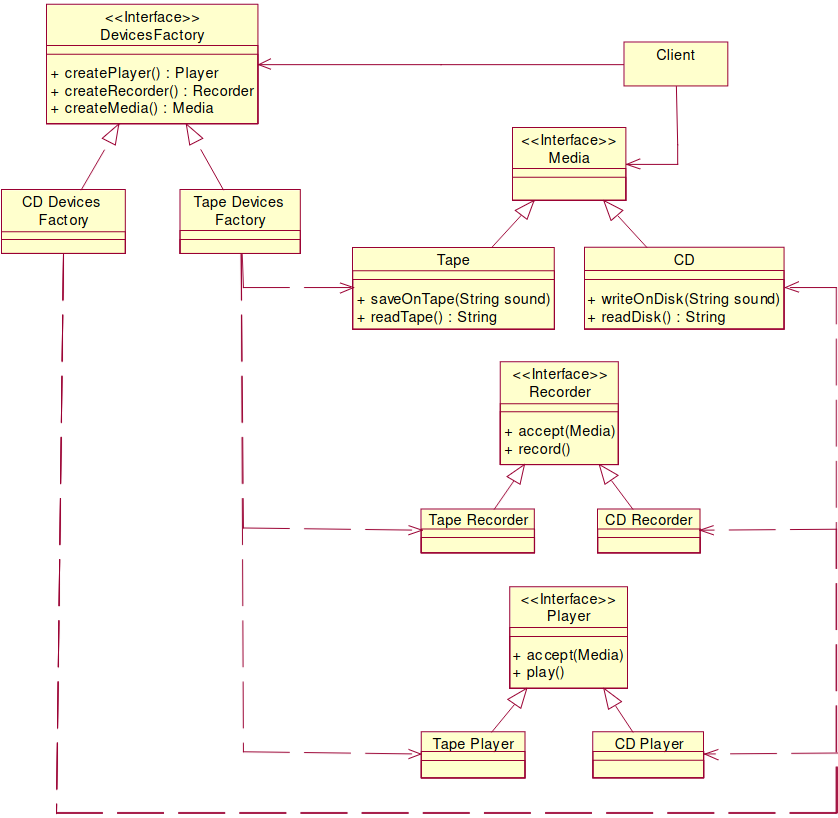
\includegraphics[scale=0.37]{images/Applicazione di Factory.png}
    \end{center}
}


\subsection{Singleton}

\mypattern{Singleton}{
    
        \paragraph{Problema:} È consentita (o richiesta) esattamente una sola istanza di una classe, ovvero un
        “singleton”. Gli altri oggetti hanno bisogno di un punto di accesso globale e
        singolo a questo oggetto.
    
        \paragraph{Soluzione:} Si definisce un metodo statico della classe
        che restituisce l'istanza della classe stessa (Singleton).
    
}

\clm{}{}{
    \begin{itemize}
        \item [$\Rightarrow$] Il Singleton definisce una classe della quale è possibile
        l'istanziazione di un unico oggetto tramite un metodo statico incaricato
        di restituire l'istanza;
        \item [$\Rightarrow$] Le diverse richieste di istanziazione restituiscono
        un riferimento allo stesso oggetto;
        \item [$\Rightarrow$] In UML viene illustrato con un "1" nella sezione del nome.
    \end{itemize}
    \paragraph{In Java ci sono tre possibili implementazioni:}
    \begin{itemize}
        \item [$\Rightarrow$] \textbf{Come classe statica:} non è un vero Singleton,
        perchè si lavora con la classe e non con l'oggetto;
        \item [$\Rightarrow$] \textbf{Creato da un metodo statico:} la prima chiamata alla classe
        crea l'oggetto, le successive restituiscono l'oggetto creato (inizializzazione \fancyglitter{pigra});
        \item [$\Rightarrow$] \textbf{Multi-thread:} versione a multi-thread della precedente.
    \end{itemize}
    \paragraph{Il Singleton creato da un metodo statico è preferibile al
    Singleton come classe statica perchè:}
    \begin{itemize}
        \item [$\Rightarrow$] I metodi d'istanza consentono la ridefinizione nelle 
        sottoclassi e il raffinamento;
        \item [$\Rightarrow$] La maggior parte dei meccanismi di comunicazione remota orientati agli oggetti supporta l'accesso remoto solo
        a metodi d'istanza;
        \item [$\Rightarrow$] Una classe non è sempre un Singleton.
    \end{itemize}
}

\cd{
    \begin{center}
        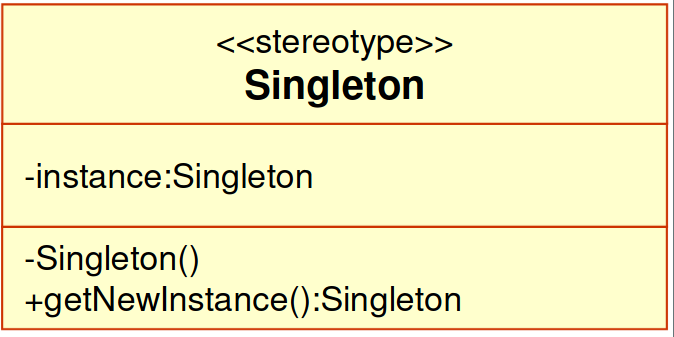
\includegraphics[scale=0.3]{images/Singleton1.png}
    \end{center}
    
}

\ex{Applicazione di Singleton}{
    \begin{center}
        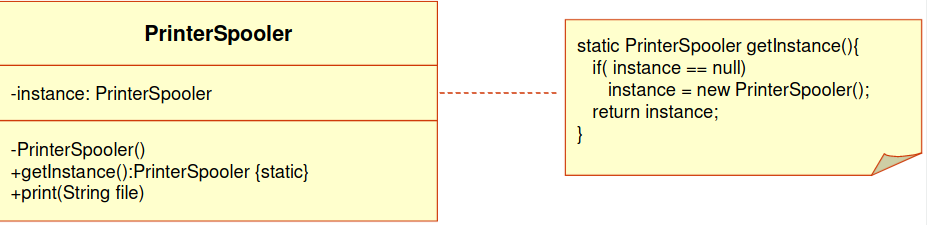
\includegraphics[scale=0.3]{images/Applicazione di Singleton.png}
    \end{center}
}

\section{Pattern Strutturali}

\dfn{Pattern Strutturali}{
    I \newfancyglitter{pattern strutturali} risolvono problematiche inerenti
    la struttura delle classi e degli oggetti.
}


\subsection{Adapter}

\mypattern{Adapter}{

    \paragraph{Problema:} Come gestire interfacce incompatibili o fornire
    un'interfaccia stabile a comportamenti simili ma con interfacce diverse?

    \paragraph{Soluzione:} Si converte l'interfaccia originale di un componente
    in un'altra interfaccia attraverso un adattatore intermedio.

}

\nt{Adapter viene spesso usato per aumentare la riusabilità del software.}

\clm{}{}{
    \begin{itemize}
        \item [$\Rightarrow$] In una coppia client-server le interfacce sono
        \fancyglitter{incompatibili} quando l'oggetto server offre servizi di 
        interesse per l'oggetto client, ma l'oggetto client vuole fruire di questi
        servizi in una modalità diversa da quella offerta dall'oggetto server;
        \item [$\Rightarrow$] Ci sono più oggetti server che offrono servizi simili, 
        che hanno interfacce simili, ma diverse. Un oggetto client vuole fruire
        dei servizi di uno di questi oggetti server (componenti simili, ma con interfacce diverse).
    \end{itemize}
    \paragraph{Generalmente:}
    \begin{enumerate}
        \item Un adattatore riceve una richiesta da un client (nel formato del client);
        \item L'adattatore converte la richiesta nel formato del server;
        \item L'adattatore inoltra la richiesta al server;
        \item Se il server fornisce una risposta lo fa nel suo formato;
        \item L'adattatore converte la risposta nel formato del client e la restituisce
        al client.
    \end{enumerate}
}

\cd{
    \begin{center}
        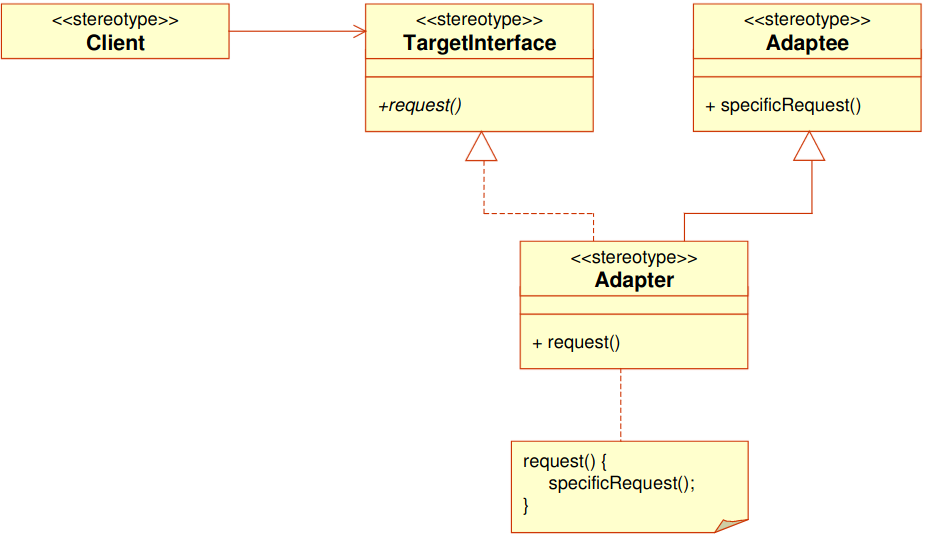
\includegraphics[scale=0.31]{images/Adapter.png}
    \end{center}
}

\ex{Applicazione di Adapter: classe}{
    \begin{center}
        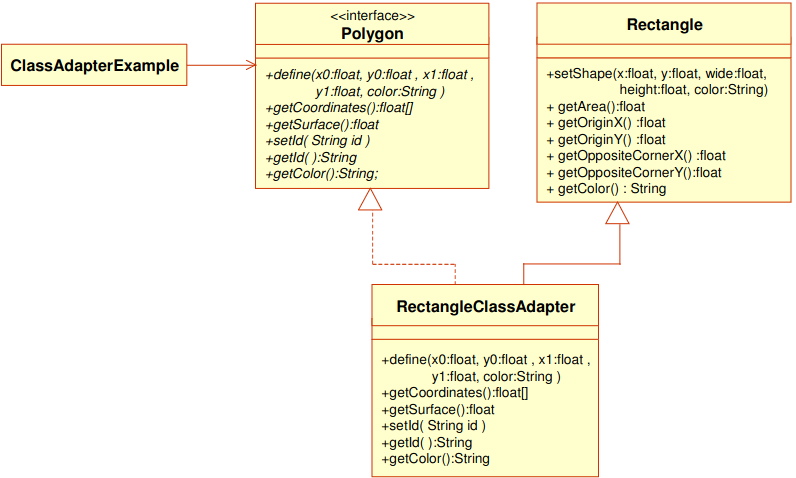
\includegraphics[scale=0.37]{images/Adapter1.png}
    \end{center}
}

\cd{
    \begin{center}
        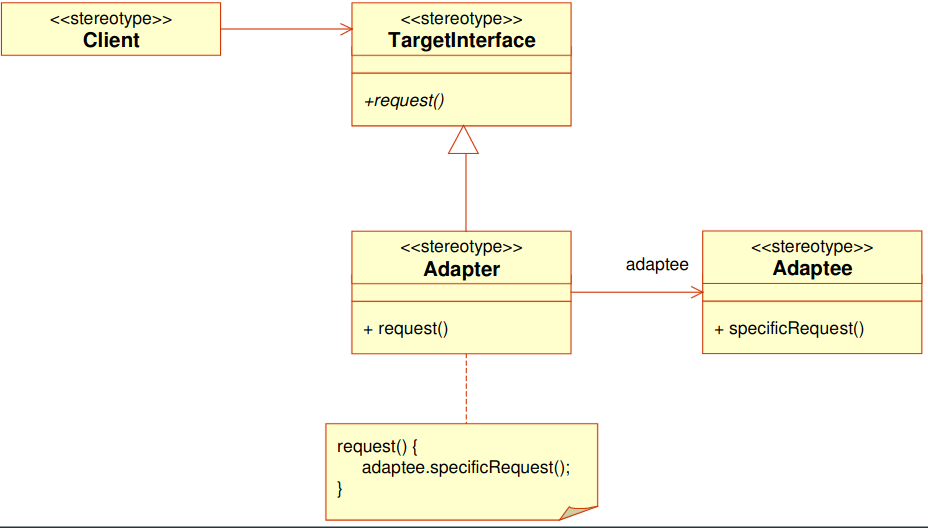
\includegraphics[scale=0.37]{images/Adapter2.png}
    \end{center}
}

\ex{Applicazione di Adapter: oggetto}{
    \begin{center}
        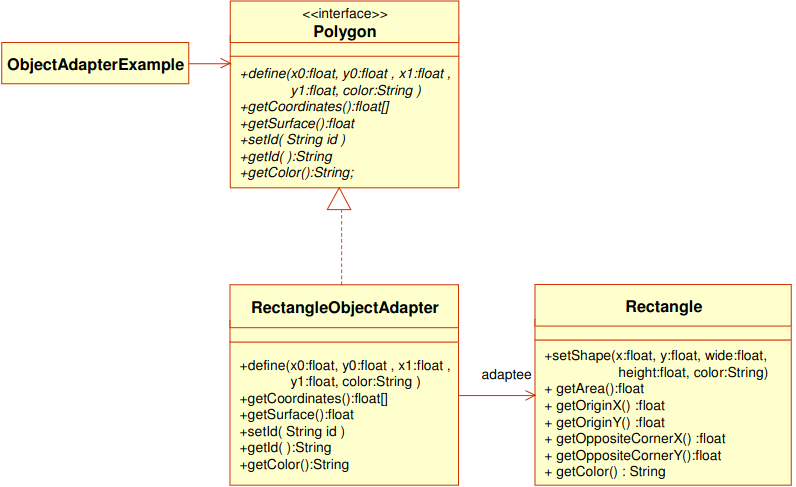
\includegraphics[scale=0.37]{images/Adapter3.png}
    \end{center}
}

\subsection{Composite}

\mypattern{Composite}{

    \paragraph{Problema:} Come trattare un gruppo o una struttura
    composta di oggetti (polimorficamente) dello stesso tipo nello stesso
    modo di un oggetto non composto (atomico)?

    \paragraph{Soluzione:} Si definiscono le classi per gli oggetti composti
    e atomici in modo che implementino la stessa intefaccia.

}

\clm{}{}{
    \begin{itemize}
        \item [$\Rightarrow$] Consente la costruzione di gerarchie di oggetti composti;
        \item [$\Rightarrow$] È anche noto come \fancyglitter{struttura ad aòbero},
        \fancyglitter{composizione ricorsiva} o \fancyglitter{struttura induttiva},
        in cui foglie e nodi hanno le stesse funzionalità.
    \end{itemize}
    \paragraph{È utile per:}
    \begin{itemize}
        \item [$\Rightarrow$] Creare gerarchie \fancyglitter{tutto-parte};
        \item [$\Rightarrow$] Ignorare le differenze tra oggetti atomici e composti;
        \item [$\Rightarrow$] Implementare la stessa interfaccia per tutti gli elementi contenuti.
    \end{itemize}
    \paragraph{Il pattern definisce una classe astratta \fancyglitter{componente} che
    deve essere estesa in due sottoclassi:}
    \begin{itemize}
        \item [$\Rightarrow$] \fancyglitter{Foglia:} rappresenta un oggetto atomico;
        \item [$\Rightarrow$] \fancyglitter{Nodo:} rappresenta un oggetto composto e si implementa 
        come contenitore di componenti.
    \end{itemize}
}

\cd{
    \begin{center}
        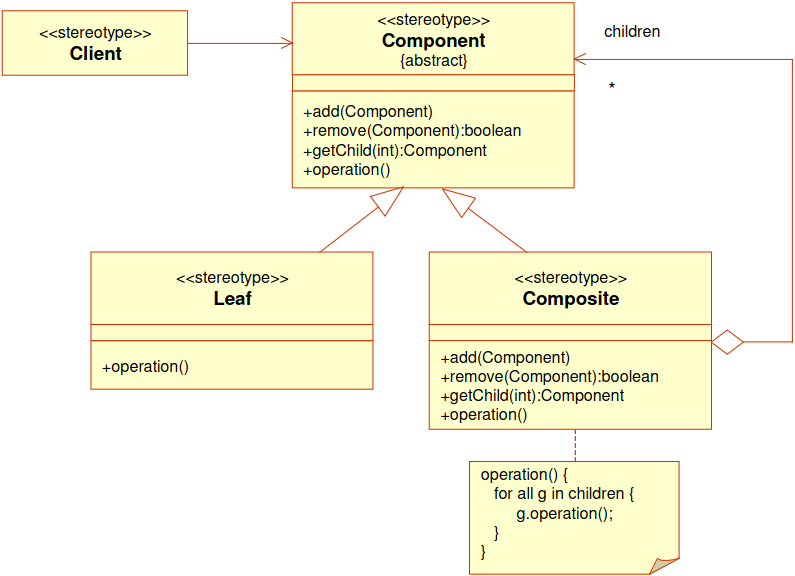
\includegraphics[scale=0.42]{images/Composite.png}
    \end{center}
}

\ex{Applicazione di Composite}{
    \begin{center}
        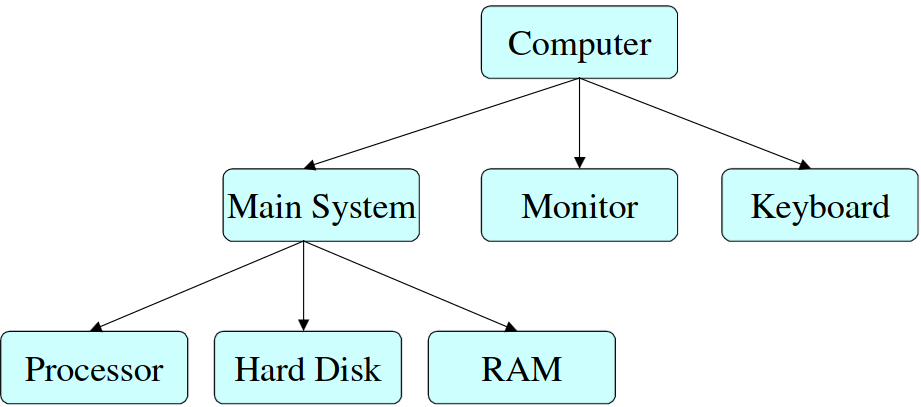
\includegraphics[scale=0.44]{images/Applicazione di Composite.png}
        \paragraph{}
        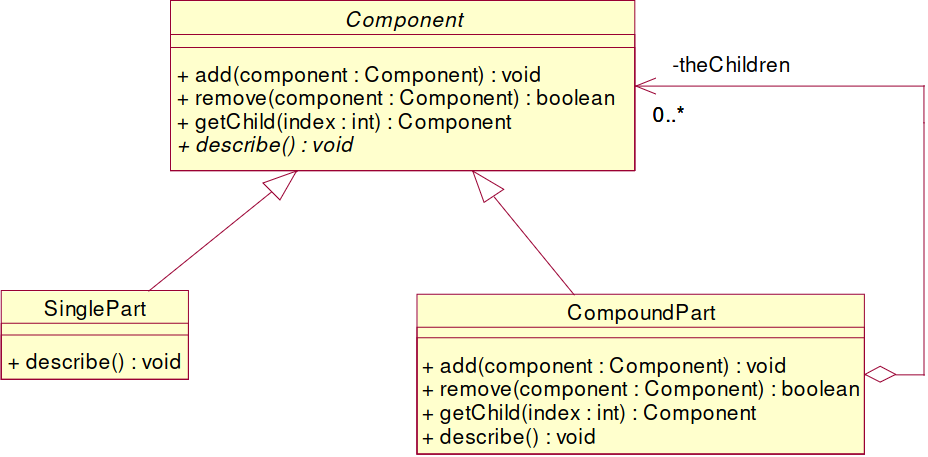
\includegraphics[scale=0.44]{images/Applicazione di Composite 2.png}
        \paragraph{}
        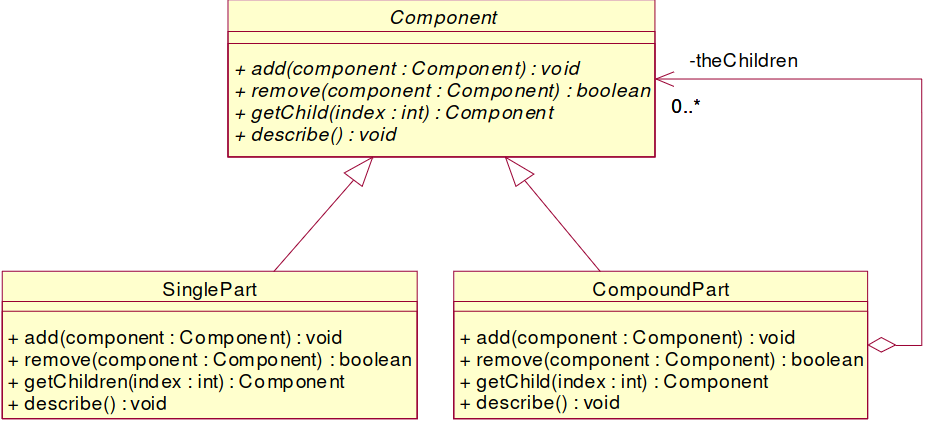
\includegraphics[scale=0.44]{images/Applicazione di Composite 1.png}
    \end{center}
}

\ex{Applicazione di composite: tree}{
    \begin{center}
        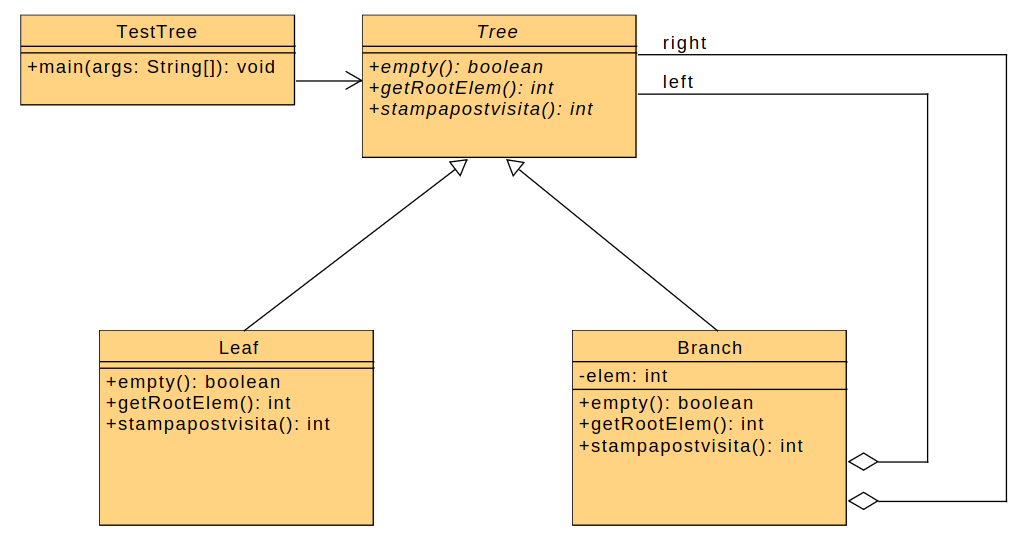
\includegraphics[scale=0.42]{images/Applicazione di Composite 3.png}
    \end{center}
}

\subsection{Decorator}

\mypattern{Decorator}{

    \paragraph{Problema:} Come permettere l'assegnamento di una o più responsabilità
    a un oggetto in maniera dinamica ed evitare il problema della relazione statica?
    Come provvedere un'alternativa più flessibile al meccanismo di sottoclasse ed evitare
    il problema di avere una gerarchia di classi complessa?

    \paragraph{Soluzione:} Si ingloba l'oggetto all'interno di un altro che
    aggiunge le nuove funzionalità.

}

\nt{Riduce l'uso di extends, di fatto "simulandolo".}

\clm{}{}{
    \begin{itemize}
        \item [$\Rightarrow$] Il Decorator è anche chiamato \fancyglitter{Wrapper};
        \item [$\Rightarrow$] È usato per aggiungere responsabilità a oggetti individualmente,
        dinamicamente e in maniera trasparente (senza impatti su altri oggetti);
        \item [$\Rightarrow$] Le responsabilità possono essere \fancyglitter{ritirate};
        \item [$\Rightarrow$] Evita l'\fancyglitter{esplosione delle sottoclassi} (evita
        la creazione di una classe per ogni combinazione di responsabilità).
    \end{itemize}
}

\cd{
    \begin{center}
        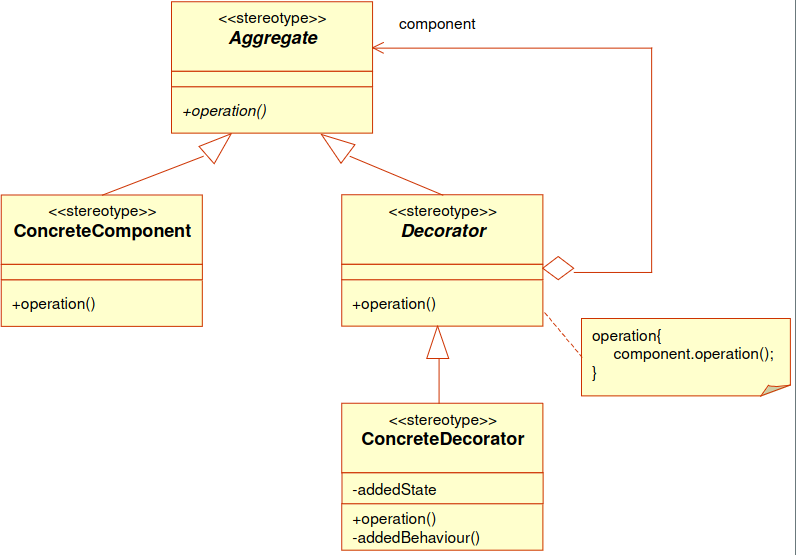
\includegraphics[scale=0.5]{images/Decorator.png}
    \end{center}
}

\ex{Applicazione di Decorator}{
    \begin{center}
        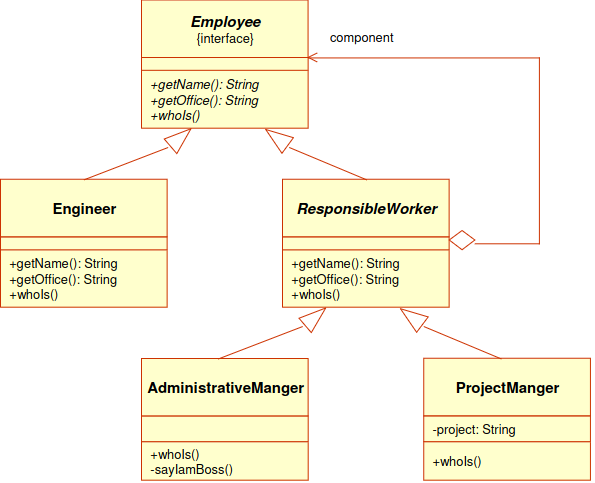
\includegraphics[scale=0.7]{images/Applicazione del Decorator.png}
    \end{center}
}

\section{Pattern Comportamentali}

\dfn{Pattern Comportamentali}{
    I \newfancyglitter{pattern comportamentali} risolvono problematiche inerenti
    riguardanti l'interazione tra oggetti.    
}

\subsection{Observer}

\mypattern{Observer}{
    \paragraph{Problema:} Diversi tipi di oggetti \textit{subscriber} (abbonato)
    sono interessati ai cambiamenti di stato o agli eventi di un oggetto \textit{publisher}
    (editore). Ciascun subscriber vuole reagire in modo suo quando il publisher genera 
    un evento. Inoltre il publisher vuole mantenere un accoppiamento basso
    (vedi \ref{LowCoupling}) verso i suoi subscriber. Cosa si deve fare?

    \paragraph{Soluzione:} Si definisce un'interfaccia subscriber o listener.
    Gli oggetti subscriber implementano questa interfaccia. Il publisher
    registra dinamicamente i subscriber che sono interessati ai suoi eventi e li 
    notifica quando avvengono.
}

\nt{Questo pattern è anche chiamato \fancyglitter{publish-subscribe} o \fancyglitter{dependents}.}

\clm{}{}{
    \begin{itemize}
        \item [$\Rightarrow$] Definisce una dipendenza uno-a-molti tra oggetti.
        Quando un oggetto cambia stato, tutti i suoi dipendenti vengono notificati;
        \item [$\Rightarrow$] L'oggetto che notifica il cambiamento di stato non
        fa nessuna assunzione sulla natura degli oggetti notificati (sono disaccoppiati);
        \item [$\Rightarrow$] Il numero degli oggetti affetti dal cambiamento di stato
        di un oggetto non è noto a priori;
        \item [$\Rightarrow$] Fornisce un modo per accoppiare in maniera debole degli oggetti
        che devono comunicare (eventi). I publisher conoscono i subscriber solo attraverso
        un'interfaccia e i subscriber possono registrarsi (o cancellarsi) dinamicamente con
        il publisher;
        \item [$\Rightarrow$] Spesso viene associato al pattern MVC.
    \end{itemize}
}

\cd{
    \begin{center}
        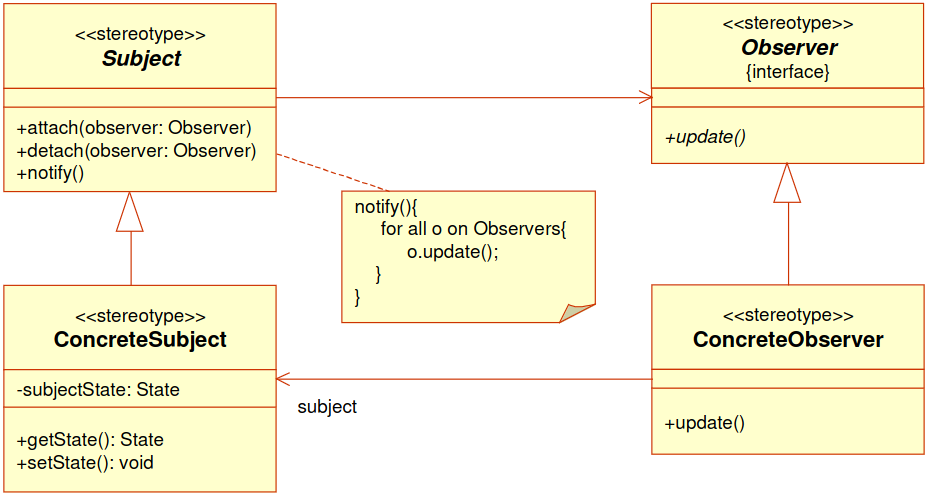
\includegraphics[scale=0.37]{images/Observer.png}
    \end{center}
}

\ex{Funzionamento di Observer}{
    \begin{center}
        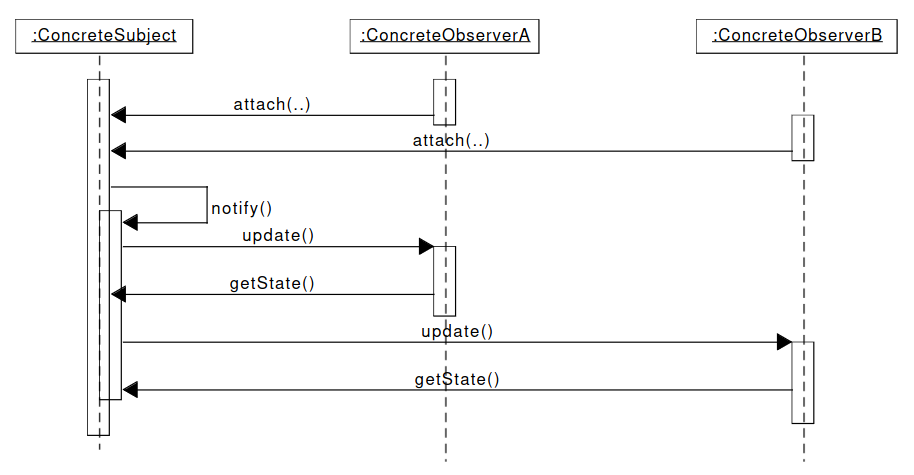
\includegraphics[scale=0.49]{images/Observer 1.png}
    \end{center}
}

\ex{Applicazione di Observer}{

    \begin{center}
        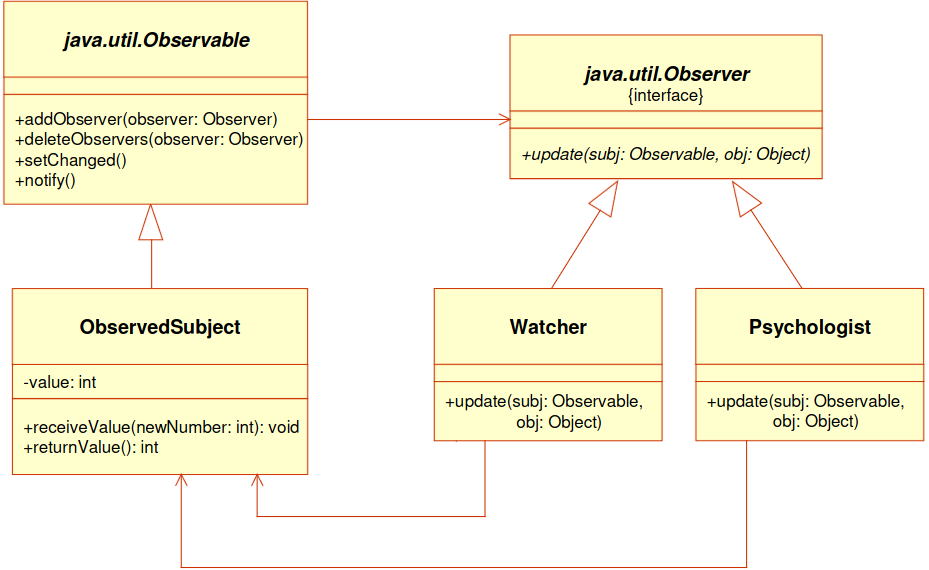
\includegraphics[scale=0.48]{images/Applicazione di Observer.png}
    \end{center}

}

\subsection{State}

\mypattern{State}{
    \paragraph{Problema:} Il comportamento di un oggetto dipende dal suo stato
    e i suoi metodi contengono logica condizionale per casi che riflette le azioni
    condizionali che dipendono dallo stato. C'è un'alternativa alla logica condizionale?

    \paragraph{Soluzione:} Si creano delle classi stato per ciascuno stato che implementano
    un'interfaccia comune. Si delegano le operazioni che dipendono dallo stato dell'oggetto
    contesto all'oggetto stato corrispondente. Si assicura che l'oggetto contesto referenzi 
    sempre un oggetto stato che riflette il suo stato corrente.
}

\clm{}{}{
    \begin{itemize}
        \item [$\Rightarrow$] Permette a un oggetto di modificare il suo comportamento
        quando il suo stato interno cambia.
    \end{itemize}
}

\cd{
    \begin{center}
        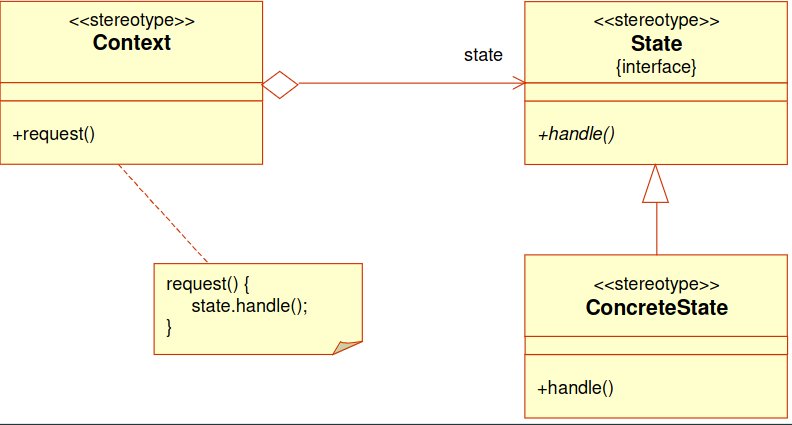
\includegraphics[scale=0.37]{images/State.png}
    \end{center}
}

\ex{Funzionamento di State}{
    \begin{center}
        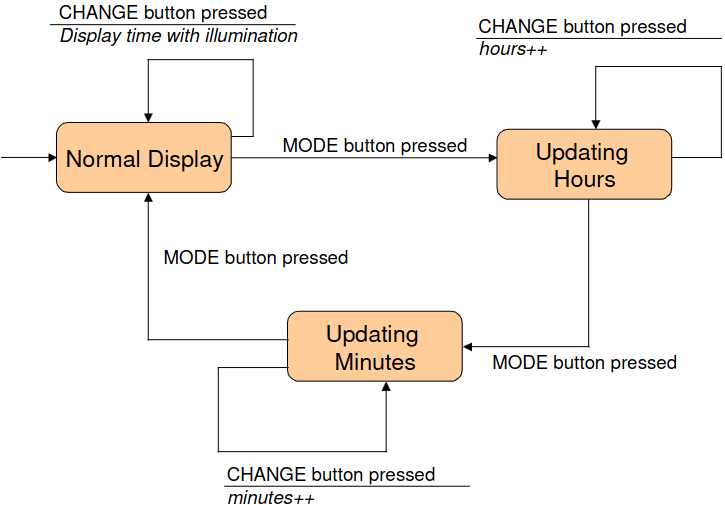
\includegraphics[scale=0.4]{images/State 1.png}
    \end{center}

}

\ex{Applicazione di State}{
    \begin{center}
        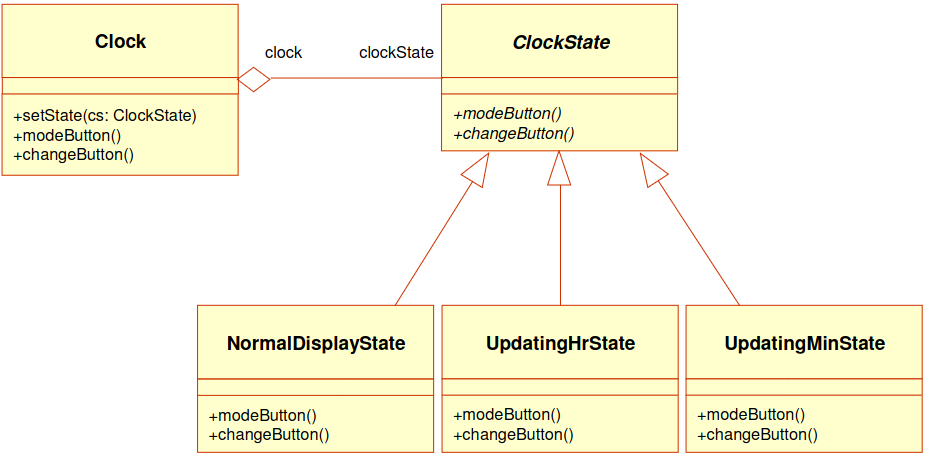
\includegraphics[scale=0.37]{images/Applicazione di State.png}
    \end{center}
}

\subsection{Strategy}

\mypattern{Strategy}{
    \paragraph{Problema:} Come progettare per gestire un insieme di algoritmi 
    o politiche variabili ma correlati? Come progettare per consentire di
    modificare questi algoritmi o politiche?

    \paragraph{Soluzione:} Si definisce ciascun algoritmo/politica/strategia in una
    classe separata, con un'interfaccia comune.
}

\nt{Il pattern Strategy è anche chiamato \fancyglitter{policy}.}

\clm{}{}{
    \begin{itemize}
        \item [$\Rightarrow$] L'oggetto contesto è l'oggetto a cui va applicato
        l'algoritmo;
        \item [$\Rightarrow$] L'oggetto contesto è associato a un oggetto strategia, che
        è l'oggetto che implementa l'algoritmo;
        \item [$\Rightarrow$] Strategy consente la definizione di una famiglia di algoritmi,
        li incapsula e li rende intercambiabili;
        \item [$\Rightarrow$] Strategy consente di variare l'algoritmo indipendentemente
        dagli oggetti che lo usano;
        \item [$\Rightarrow$] Disaccoppia gli algoritmi dai clienti che vogliono usarli dinamicamente;
        \item [$\Rightarrow$] Permette al cliente di scegliere l'algoritmo più adatto;
        \item [$\Rightarrow$] È usato per modificare il comportamento di un oggetto a tempo di esecuzione;
        \item [$\Rightarrow$] Usa la composizione invece dell'ereditarietà.
    \end{itemize}
}

\cd{
    \begin{center}
        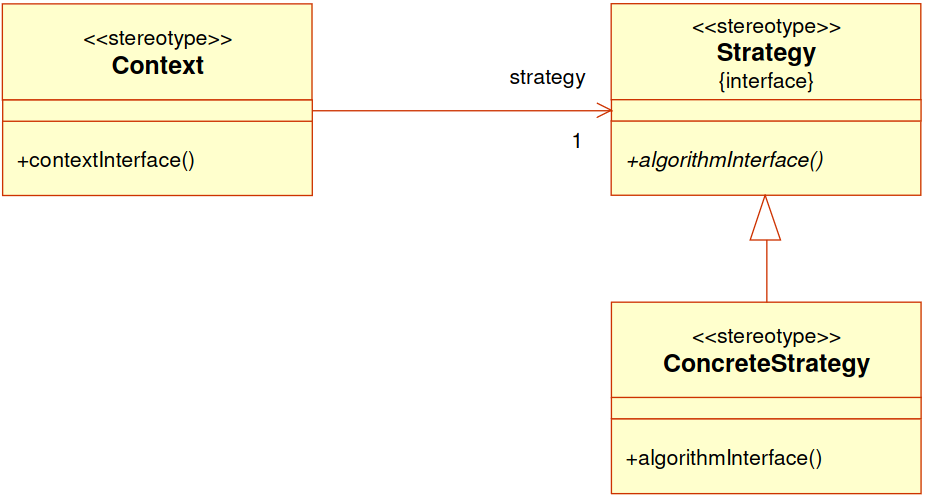
\includegraphics[scale=0.42]{images/Strategy.png}
    \end{center}
}

\ex{Applicazione di Strategy}{
    \begin{center}
        \includegraphics[scale=0.45]{images/Applicazione di Strategy.png}
    \end{center}
}

\cor{Strategy e State}{
    \begin{itemize}
        \item [$\Rightarrow$] State si occupa di che cosa (stato o tipo) un oggetto è 
        (al suo interno) e incapsula un comportamento che dipende dallo stato;
        \item [$\Rightarrow$] Strategy si occupa di come un oggetto fa qualcosa e incapsula
        un algoritmo. Un'implementazione diversa che realizza la stessa cosa, in modo che
        un'implementazione possa sostituire l'altra a seconda della strategia richiesta.
    \end{itemize}
}

\subsection{Visitor}

\mypattern{Visitor}{
    \paragraph{Problema:} Come separare l'operazione applicata su un contenitore
    complesso dalla struttura dati cui è applicata? Come poter aggiungere nuove
    operazioni e comportamenti senza dover modificare la struttura stessa?
    Come attraversare il contenitore complesso i cui elementi sono eterogenei
    applicando azioni dipendenti dal tipo degli elementi?

    \paragraph{Soluzione:} Si crea un oggetto (ConcreteVisitor) che è in grado di
    percorrere la collezione, e di applicare un metodo proprio su un oggetto (Element)
    visitato nella collezione (avendo un riferimento a questi ultimi come parametro).
    Ogni oggetto della collezione aderisce a un'interfaccia (Visitable) che consente al 
    ConcreteVisitor di essere accettato da parte di ogni Element. Il Visitor analizza 
    il tipo di oggetto ricevuto, fa l'invocazione alla particolare operazione che
    deve eseguire.
}

\clm{}{}{
    \paragraph{Visitor consente:}
    \begin{itemize}
        \item [$\Rightarrow$] Flessibilità delle operazioni;
        \item [$\Rightarrow$] Organizzazione logica;
        \item [$\Rightarrow$] Vista di vari tipi di classi;
        \item [$\Rightarrow$] Mantenimento di uno stato aggiornabile;
        \item [$\Rightarrow$] Le diverse modalità di vista della struttura
        possono essere definite come sottoclassi di Visitor.
    \end{itemize}
}

\cd{
    \begin{center}
        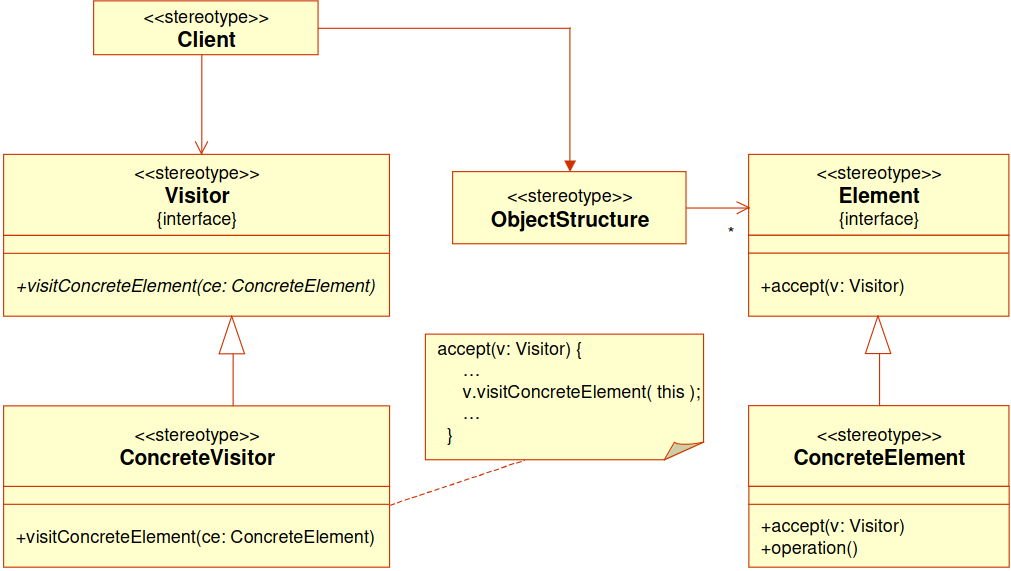
\includegraphics[scale=0.42]{images/Visitor.png}
    \end{center}

    \nt{La linea tratteggiata della \textit{accept} in realtà 
    deve essere collegata a \textit{ConcreteElement}.}
}

\ex{Applicazione di Visitor}{
    \begin{center}
        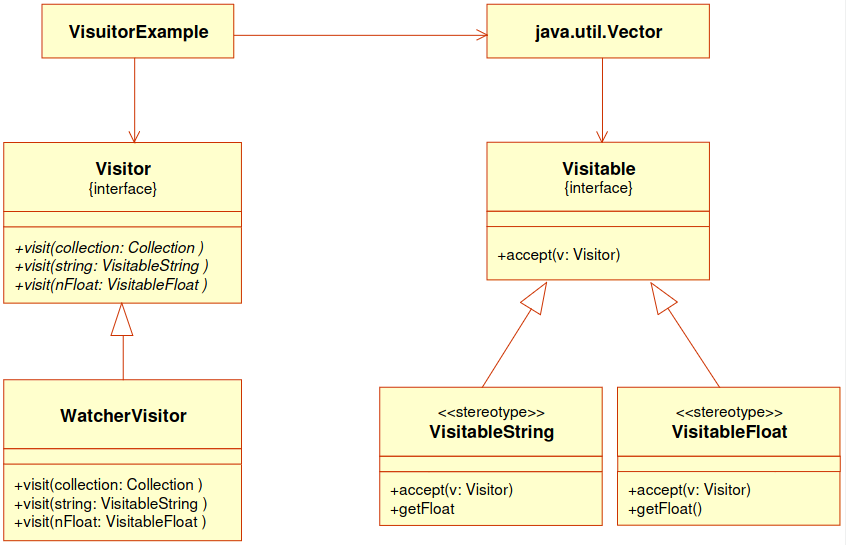
\includegraphics[scale=0.45]{images/Applicazione di Visitor.png}
    \end{center}

    \nt{Nella classe VisitableString \textit{getFloat} è \textit{getString}. }
} 




